\whiteBGstarBegin

\begin{enumerate}[label=\bfseries Câu \arabic*:]
	
	\item \mkstar{1}
	
	\cauhoi{Trong một mạch kín gồm nguồn điện có suất điện động $\calE$, điện trở trong $r$ và mạch ngoài có điện trở $R$. Hệ thức nêu lên mối quan hệ giữa các đại lượng trên với cường độ dòng điện $I$ chạy trong mạch là
		\begin{mcq}(4)
			\item $I =\dfrac{\calE}{R}$.
			\item $I = \calE \sqrt{\dfrac{\calE}{R}}$.
			\item $I =\dfrac{\calE}{R+r}$.
			\item $I =\dfrac{\calE}{r}$.
		\end{mcq}
	}
	
	\loigiai{\textbf{Đáp án: C.}
		
		Định luật ôm đối với toàn mạch: Cường độ dòng điện chạy trong mạch điện kín tỉ lệ thuận với suất điện động của nguồn điện và tỉ lệ nghịch với điện trở toàn phần của mạch đó:
		$$I=\dfrac{\calE}{R+r}$$
		Với $R$ là điện trở mạch ngoài; $r$ là điện trở trong của nguồn điện.
		
		
		
	}
	\item \mkstar{1}
	
	\cauhoi{Tìm phát biểu \textbf{sai}.
		\begin{mcq}
			\item Hiện tượng đoản mạch xảy ra khi điện trở của mạch ngoài rất nhỏ.
			\item Suất điện động $\calE$ của nguồn điện luôn có giá trị bằng điện thế mạch trong.
			\item Suất điện động $\calE$ của nguồn điện có giá trị bằng độ giảm thế ở mạch ngoài và mạch trong.
			\item Điện trở toàn phần của toàn mạch là tổng giá trị số của điện trở trong và điện trở tương đương của mạch ngoài.
		\end{mcq}
	}
	
	\loigiai{\textbf{Đáp án: B.}
		
		Độ giảm thế trên đoạn mạch:
		$$U = IR$$
		Suất điện động của nguồn điện:
		$$\calE =IR + Ir > U$$
		
		
	}
	\item \mkstar{1}
	
	\cauhoi{Trong mạch điện kín gồm nguồn điện có suất điện động $\calE$, điện trở trong $r$ và mạch ngoài có điện trở $R$. Khi có hiện tượng đoản mạch thì cường độ dòng điện trong mạch $I$ được xác định bằng công thức:
		\begin{mcq}(4)
			\item $I=\dfrac{\calE}{r}$.
			\item $I=\calE r$.
			\item $I =\dfrac{r}{\calE}$.
			\item $I =\dfrac{\calE}{R+r}$.
		\end{mcq}
	}
	
	\loigiai{\textbf{Đáp án: A.}
		
		Định luật ôm đối với toàn mạch:
		$$I =\dfrac{\calE}{R+r}$$
		Khi có hiện tượng đoản mạch ($R = 0$) thì cường độ dòng điện trong mạch là
		$$I = \dfrac{\calE}{r}$$
		
		
		
	}
		\item \mkstar{1}

\cauhoi{Hạt tải điện trong kim loại là
	\begin{mcq}(2)
		\item ion dương.
		\item electron tự do.
		\item ion âm. 
		\item ion dương, ion âm, electron tự do.
	\end{mcq}
}
\loigiai{	\textbf{Đáp án: B}.
	
	Hạt tải điện trong kim loại là các electron tự do.
}
\item \mkstar{1}

\cauhoi{Trong các nhận định sau, nhận định nào về dòng điện trong kim loại là \textbf{không} đúng?
	\begin{mcq}
		\item  	Nguyên nhân điện trở của kim loại là do sự mất trật tự trong mạng tinh thể.
		\item 	Khi trong kim loại có dòng điện thì electron sẽ chuyển động cùng chiều điện trường.
		\item   Nhiệt độ của kim loại càng cao thì dòng điện qua nó bị cản trở càng nhiều.
		\item 	Dòng điện trong kim loại là dòng chuyển dời có hướng của các electron tự do
	\end{mcq}
}
\loigiai{	\textbf{Đáp án: B}.  
	
	Khi trong kim loại có dòng điện thì electron sẽ chuyển động ngược chiều điện trường. 
}
	\item \mkstar{1}

\cauhoi{Hiện tượng siêu dẫn là hiện tượng
	\begin{mcq}
		\item  	điện trở của vật giảm xuống bằng không khi nhiệt độ của vật nhỏ hơn một giá trị nhiệt độ nhất định.
		\item điện trở của vật bằng không khi nhiệt độ bằng 0 K.
		\item  		điện trở của vật giảm xuống rất nhỏ khi điện trở của nó đạt giá trị đủ cao.	
		\item điện trở của vật dẫn giảm xuống giá trị rất nhỏ khi nhiệt độ giảm xuống thấp.
	\end{mcq}
}
\loigiai{\textbf{Đáp án: A}.
	
	Hiện tượng siêu dẫn là hiện tượng điện trở của vật giảm xuống bằng không khi nhiệt độ của vật nhỏ hơn một giá trị nhiệt độ nhất định.
}
\item \mkstar{1}

\cauhoi{Suất nhiệt điện động của của một cặp nhiệt điện phụ thuộc vào
	\begin{mcq}
		\item  	bản chất của chỉ một trong hai kim loại cấu tạo nên cặp.
		\item  hiệu nhiệt độ hai đầu cặp.
		\item  	nhiệt độ cao hơn ở một trong hai đầu cặp.	
		\item nhiệt độ thấp hơn ở một trong hai đầu cặp.
	\end{mcq}
}
\loigiai{\textbf{Đáp án: B}. 
	
	Suất nhiệt điện động của của một cặp nhiệt điện phụ thuộc vào hiệu nhiệt độ hai đầu cặp.
}
	\item \mkstar{1}

\cauhoi{Chọn câu đúng.
	\begin{mcq}
		\item  	Để có dòng nhiệt điện, chỉ cần duy trì sự chênh lệch nhiệt độ giữa hai dây dẫn trong cặp nhiệt điện.
		\item Khi ở trạng thái siêu dẫn, khả năng dẫn điện của dây dẫn kim loại là rất kém.
		\item  Cặp nhiệt điện được cấu tạo từ hai vật dẫn khác về bản chất, được tiếp xúc điện với nhau.
		\item Điện trở suất của kim loại giảm khi nhiệt độ kim loại tăng.
	\end{mcq}
}
\loigiai{	\textbf{Đáp án: C}. 
	
	Cặp nhiệt điện được cấu tạo từ hai vật dẫn khác về bản chất, được tiếp xúc điện với nhau.
}
		 \item \mkstar{1}

\cauhoi{Trong các chất sau, chất \textbf{không} phải chất điện phân là
	\begin{mcq} (2)
		\item  	 nước nguyên chất. 
		\item dung dịch muối ăn.
		\item  dung dịch axit nitric. 
		\item dung dịch natri hiđroxit. 
	\end{mcq}
}
\loigiai{	\textbf{Đáp án: A}.
	
	Nước nguyên chất không phải là chất điện phân.
}
\item \mkstar{1}

\cauhoi{Chọn phát biểu sai.
	\begin{mcq}
		\item  Hạt tải điện trong chất điện phân là ion dương và ion âm. 
		\item Khối lượng chất giải phóng ở điện cực của bình điện phân tỉ lệ với thời gian điện phân. 
		\item  Đương lượng điện hóa của chất giải phóng ở điện cực của bình điện phân tỉ lệ với cường độ dòng điện qua bình điện phân.
		\item Khối lượng chất giải phóng ở điện cực của bình điện phân tỉ lệ với cường độ dòng điện qua bình điện phân. 
	\end{mcq}
}
\loigiai{	\textbf{Đáp án: C}. 
	
	Đương lượng điện hóa của chất giải phóng ở điện cực của bình điện phân không tỉ lệ với cường độ dòng điện qua bình điện phân.
}
\item \mkstar{1}

\cauhoi{Hiện tượng điện phân không ứng dụng để
	\begin{mcq}(2)
		\item  đúc điện. 
		\item mạ điện.
		\item luyện nhôm.
		\item sơn tĩnh điện.
	\end{mcq}
}
\loigiai{	\textbf{Đáp án: D}.
	
	Hiện tượng điện phân không ứng dụng để sơn tĩnh điện.
}


\item \mkstar{1}

\cauhoi{Công thức nào sau đây là công thức đúng của định luật Fa-ra-đây thứ hai?
	Trong đó, $A$ là khối lượng mol, $I$ là cường độ dòng điện, $t$ là thời gian điện phân, $F$ là hằng số Fa-ra-đây, $n$ là hóa trị của chất bị điện phân.
	\begin{mcq}(2)
		\item $m=\dfrac{A\cdot I^2\cdot t}{F\cdot n}$.
		\item $m=\dfrac{A\cdot I\cdot t}{F\cdot n}$.
		\item $m=\dfrac{A\cdot I\cdot n}{F\cdot t}$.
		\item $m=\dfrac{A\cdot t\cdot n}{F\cdot I}$.
	\end{mcq}
}
\loigiai{	\textbf{Đáp án: B}.
	
	Định luật Fa-ra-đây thứ hai là: $m=\dfrac{A\cdot I\cdot t}{F\cdot n}$.
}
	\item \mkstar{1}

\cauhoi{Bản chất dòng điện trong chất khí là
	\begin{mcq}
		\item  dòng chuyển dời có hướng của các ion dương theo chiều điện trường và các ion âm ngược chiều điện trường.
		\item dòng chuyển dời có hướng của các ion dương theo chiều điện trường và các ion âm, electron ngược chiều điện trường.
		\item dòng chuyển dời có hướng của các ion dương theo chiều điện trường và các electron ngược chiều điện trường.
		\item dòng chuyển dời có hướng của các electron theo ngược chiều điện trường.
	\end{mcq}
}
\loigiai{	\textbf{Đáp án: B}. 
	
	Bản chất dòng điện trong chất khí là dòng chuyển dời có hướng của các ion dương theo chiều điện trường và các ion âm, electron ngược chiều điện trường.
}
	\item \mkstar{1}

\cauhoi{Trong không khí có ion tự do. Nếu đặt một điện trường trong không khí thì các ion di chuyển như thế nào?
	\begin{mcq}
		\item  ion âm sẽ di chuyển từ điểm có điện thế thấp đến điểm có điện thế cao.
		\item ion âm sẽ di chuyển từ điểm có điện thế cao đến điểm có điện thế thấp.
		\item các ion không di chuyển.
		\item ion dương sẽ di chuyển từ điểm có điện thế thấp đến điểm có điện thế cao.
	\end{mcq}
}
\loigiai{	\textbf{Đáp án: A}.
	
	Trong không khí có ion tự do. Nếu đặt một điện trường trong không khí thì các ion âm sẽ di chuyển từ điểm có điện thế thấp đến điểm có điện thế cao.
}
\item \mkstar{1}

\cauhoi{Hiện tượng nào sau đây \textbf{không} phải hiện tượng phóng điện trong chất khí? 
	\begin{mcq}(2)
		\item  sét.
		\item dòng điện chạy qua thủy ngân.
		\item đánh lửa ở bugi. 
		\item hồ quang điện.
	\end{mcq}
}
\loigiai{	\textbf{Đáp án: B}.
	
	Dòng điện chạy qua thủy ngân không phải là hiện tượng phóng điện trong chất khí.
}
\item \mkstar{1}

\cauhoi{Hồ quang điện được ứng dụng trong	
	\begin{mcq}(4)
		\item  hàn điện.
		\item động cơ điện.
		\item động cơ nhiệt.
		\item sơn tĩnh điện.
	\end{mcq}
}
\loigiai{	\textbf{Đáp án: A}.
	
	Hồ quang điện được ứng dụng trong hàn điện.
}
	\item \mkstar{2}
	
	\cauhoi{Cho mạch điện như hình vẽ, biết $R = r$ và suất điện động của nguồn là $\calE$. Cường độ dòng điện chạy trong mạch là
		\begin{center}
			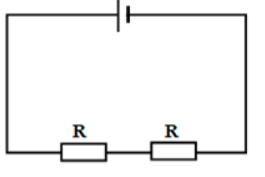
\includegraphics[scale=0.8]{../figs/VN12-Y21-PH-SYL-009-2.jpg}
		\end{center}
		\begin{mcq}(4)
			\item $I=\dfrac{2\calE}{r}$.
			\item $I=\dfrac{\calE}{3r}$.
			\item $I=\dfrac{3\calE}{2r}$.
			\item $I=\dfrac{\calE}{2r}$.
		\end{mcq}
	}
	
	\loigiai{\textbf{Đáp án: B.}	
		
		Định luật ôm đối với toàn mạch:
		$$I=\dfrac{\calE}{R+R+r} = \dfrac{\calE}{2r+r} = \dfrac{\calE}{3r}$$
		
		
	}
	\item \mkstar{2}
	
	\cauhoi{Cho mạch điện như hình vẽ, bỏ qua điện trở các đoạn dây nối. Biết $R_1 = 3\ \Omega, R_2 = 6\ \Omega, R_3 = 1\ \Omega, \calE = 6\ \text{V}, r = 1\ \Omega$. Cường độ dòng điện qua mạch chính là
		\begin{center}
			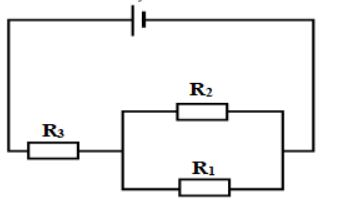
\includegraphics[scale=0.8]{../figs/VN12-Y21-PH-SYL-009-3.jpg}
		\end{center}
		\begin{mcq}(4)
			\item 0,5 A.
			\item 1 A.
			\item 1,5 A.
			\item 2 A.
		\end{mcq}
	}
	
	\loigiai{\textbf{Đáp án: C.}
		
		Cường độ dòng điện qua mạch chính:
		$$I =\dfrac{\calE}{r + R_3 + \dfrac{R_1R_2}{R_1+R_2}}=\text{1,5}\ \text{A}$$
		
		
	}
	\item \mkstar{2}
	
	\cauhoi{Hai nguồn điện giống nhau, mỗi nguồn có suất điện động là 2 V, điện trở trong là $1\ \Omega$, được mắc song song với nhau và nối với một điện trở ngoài $R$. Điện trở $R$ bằng bao nhiêu để cường độ dòng điện đi qua nó là 1 A?
		\begin{mcq}(4)
			\item $\text{1,5}\ \Omega$.
			\item $1\ \Omega$.
			\item $2\ \Omega$.
			\item $3\ \Omega$.
		\end{mcq}
	}
	
	\loigiai{\textbf{Đáp án: A.}
		
		Suất điện động của nguồn 
		$$\calE_\text{b} = \calE = 2\ \text{V}$$
		Điện trở trong của nguồn
		$$r_\text{b}=\dfrac{r}{2} = \text{0,5}\ \Omega$$
		Cường độ dòng điện đi qua $R$ là
		$$I=\dfrac{\calE_\text{b}}{R+r_\text{b}} = 1 \Rightarrow R =\text{1,5}\ \Omega$$
		
		
	}
	\item \mkstar{2}
	
	\cauhoi{Có 8 nguồn điện cùng loại với cùng suất điện động $\calE = 2\ \text{V}$ và điện trở trong $r = 1\ \Omega$. Mắc các nguồn thành bộ hỗn hợp đối xứng gồm hai dãy song song. Suất điện động $\calE_\text{b}$ và điện trở trong $r_\text{b}$ của bộ này bằng
		\begin{mcq}(2)
			\item $\calE_\text{b}=4\ \text{V}; r_\text{b}=2\ \Omega$.
			\item $\calE_\text{b}=6\ \text{V}; r_\text{b}=4\ \Omega$.
			\item $\calE_\text{b}=6\ \text{V}; r_\text{b}=1\ \Omega$.
			\item $\calE_\text{b}=8\ \text{V}; r_\text{b}=2\ \Omega$.
		\end{mcq}
	}
	
	\loigiai{\textbf{Đáp án: D.}
		
		Suất điện động của bộ nguồn:
		$$\calE_\text{b} =4\calE =8\ \text{V}.$$
		Điện trở trong của bộ nguồn:
		$$r_\text{b} = \dfrac{4r}{2} =2r=2\ \Omega.$$
		
		
	}
	\item \mkstar{2}
	
	\cauhoi{Có ba pin giống nhau, mỗi pin có suất điện động $\calE$ và điện trở trong $r$. Suất điện động và điện trở trong của bộ pin ghép song song là
		\begin{mcq} (4)
			\item $\calE$ và $\dfrac{r}{3}$.
			\item $3\calE$ và $3r$.
			\item $2\calE$ và $\dfrac{3r}{2}$.
			\item $\calE$ và $\dfrac{r}{2}$.
		\end{mcq}
	}
	
	\loigiai{\textbf{Đáp án: A.}
		
		3 pin ghép song song:
		$$\calE_\text{b} =\calE.$$
		và 
		$$r_\text{b} = \dfrac{r}{n} =\dfrac{r}{3}$$
		
		
	}
	\item \mkstar{2}
	
	\cauhoi{Có bốn nguồn giống nhau mắc nối tiếp, mỗi nguồn có suất điện động $\calE$ và điện trở trong $r$. Khi đó suất điện động và điện trở trong bộ nguồn này là
		\begin{mcq}(4)
			\item $\calE, r$.
			\item $2\calE, 2r$.
			\item $4\calE, \dfrac{r}{4}$.
			\item $4\calE, 4r$.
		\end{mcq}
	}
	
	\loigiai{\textbf{Đáp án: D.}
		
		4 nguồn mắc nối tiếp
		$$\calE_\text{b} =4\calE.$$
		và 
		$$r_\text{b} = 4r$$
		
		
		
	}
	\item \mkstar{2}
	
	\cauhoi{Có 24 nguồn điện giống nhau, suất điện động và điện trở trong của mỗi nguồn là $\calE = \text{1,5}\ \text{V}$ và $r = \text{0,5}\ \Omega$, mắc hỗn hợp đối xứng thành bốn dãy song song với nhau (mỗi dãy có sáu nguồn điện mắc nối tiếp). Suất điện động và điện trở trong của bộ nguồn là
		\begin{mcq}(2)
			\item 6 V và 0,75 $\Omega$.
			\item 9 V và 1,5 $\Omega$.
			\item 6 V và 1,5 $\Omega$. 
			\item 9 V và 0,75 $\Omega$.
		\end{mcq}
	}
	
	\loigiai{\textbf{Đáp án: D.}
		
		4 dãy mỗi dãy có 6 nguồn điện mắc nối tiếp
		$$\calE_\text{b} =6\calE=9\ \text{V}.$$
		và 
		$$r_\text{b} = \dfrac{6r}{4}=\text{0,75}\ \Omega$$
		
		
	}
	\item \mkstar{2}
	
	\cauhoi{Có ba nguồn giống nhau có suất điện động $\calE$ và điện trở trong $r$ mắc thành bộ như hình vẽ. Điều nào sau đây là đúng với bộ nguồn ($\calE$, $r_\text{b}$)?
		\begin{center}
			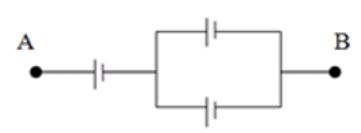
\includegraphics[scale=0.8]{../figs/VN12-Y21-PH-SYL-009-4.jpg}
		\end{center}
		\begin{mcq}(2)
			\item $3\calE; 3r$.
			\item $\text{1,5}\calE; \text{1,5}r$.
			\item $2\calE; \text{1,5}r$.
			\item $\calE; r$.
		\end{mcq}
	}
	
	\loigiai{\textbf{Đáp án: C.}
		
		Ta có:
		$$\calE_\text{b} =\calE + \calE =2\calE .$$
		và 
		$$r_\text{b} = r+\dfrac{r}{2}=\text{1,5}r$$
		
		
	}
	\item \mkstar{2}

\cauhoi{Kim loại dẫn điện tốt vì
	\begin{mcq}
		\item  giá trị điện tích chứa trong mỗi electron tự do của kim loại lớn hơn ở các chất khác.
		\item 	khoảng cách giữa các ion nút mạng trong kim loại rất lớn.
		\item   mật độ electron tự do trong kim loại rất lớn.
		\item 	mật độ các ion tự do lớn.
	\end{mcq}
}
\loigiai{	\textbf{Đáp án: C}. 
	
	Kim loại dẫn điện tốt vì mật độ electron tự do trong kim loại rất lớn.
}
\item \mkstar{2}

\cauhoi{Câu nào dưới đây nói về tính chất điện của kim loại là không đúng?
	\begin{mcq}
		\item  Kim loại là chất dẫn điện. 
		\item Điện trở suất của kim loại thường rất lớn. 
		\item Điện trở suất của kim loại tăng khi nhiệt độ tăng.
		\item Cường độ dòng điện chạy qua dây dẫn kim loại tuân theo đúng định luật Ohm khi nhiệt độ của dây kim loại thay đổi không đáng kể.
	\end{mcq}
}
\loigiai{	\textbf{Đáp án: B}.
	
	Điện trở suất của kim loại thường nhỏ, nhỏ hơn $10^{-7 }\ \Omega \text{m}$. 
}

\item \mkstar{2}

\cauhoi{Ở $20^\circ \text{C}$ điện trở suất của bạc là $\text{1,62}\cdot 10^{-8}\ \Omega\cdot \text{m}$. Biết hệ số nhiệt điện trở của bạc là là $\text{4,1}\cdot 10^{-3}\, \text{K}^{-1}$. Ở 300 K thì điện trở suất của bạc là 
	\begin{mcq}(2)
		\item $\text{1,67}\cdot 10^{-6}\ \Omega\cdot \text{m}$. 
		\item $\text{1,67}\cdot 10^{-4}\ \Omega\cdot \text{m}$. 
		\item $\text{1,67}\cdot 10^{-8}\ \Omega\cdot \text{m}$.
		\item $\text{1,67}\cdot 10^{-2\ }\Omega\cdot \text{m}$.
	\end{mcq}
}
\loigiai{	\textbf{Đáp án: C}.
	
	$\rho = \rho_o \left( 1+\alpha\left( t-t_\text{0}\right) \right)= \text{1,67}\cdot 10^{-8}\ \Omega\cdot \text{m}$.
}
	\item \mkstar{2}

\cauhoi{Chọn câu đúng.
	\begin{mcq}
		\item  	Cặp nhiệt điện là hai dây kim loại khác bản chất, hai đầu hàn vào nhau.
		\item Cặp nhiệt điện là hai dây kim loại cùng bản chất, hai đầu hàn vào nhau.
		\item  Cặp nhiệt điện là hai dây cách điện khác bản chất, hai đầu hàn vào nhau.	
		\item Cặp nhiệt điện gồm một dây kim loại và một dây cách điện, hai đầu hàn vào nhau.
	\end{mcq}
}
\loigiai{\textbf{Đáp án: A}.  
	
	Cặp nhiệt điện là hai dây kim loại khác bản chất, hai đầu hàn vào nhau.				
}
	\item \mkstar{2}

\cauhoi{Nối cặp nhiệt đồng – constantan với một milivôn kế thành một đoạn mạch kín. Nhúng mối hàn thứ nhất vào nước đá đang tan và mối hàn thứ hai vào hơi nước sôi, milivôn kế chỉ $\text{4,25}$. Tính hệ số nhiệt điện động của cặp nhiệt điện. 
	\begin{mcq}(2)
		\item  	$ \text{4,25}\cdot 10^{-5}\  \text{V/ K}$.
		\item $ \text{4,25}\cdot 10^{5}\  \text{V/ K}$.
		\item  	$ \text{4,25}\cdot 10^{-2}\  \text{V/ K}$.	
		\item $ \text{4,25}\cdot 10^{-3}\  \text{V/ K}$.
	\end{mcq}
}
\loigiai{\textbf{Đáp án: A}.
	
	$\calE = \alpha _T (T_2-T_1)$
	$\Rightarrow  \alpha_T= \text{4,25}\cdot 10^{-5}\  \text{V/ K}$.
}
	\item \mkstar{2}

\cauhoi{Một cặp nhiệt điện có hệ số nhiệt điện động là $\text{8,6}\ \mu \text{V}\cdot \text K^{-1}$. Suất điện động là $\text{17,2}\ \text{mV}$. Tính nhiệt độ chênh lệch giữa hai đầu của cặp nhiệt điện.
	\begin{mcq}(4)
		\item $200^\circ\text{C}$.
		\item $2000^\circ\text{C}$.
		\item $20^\circ \text{C}$.
		\item $20000^\circ \text{C}$.
	\end{mcq}
}
\loigiai{	\textbf{Đáp án: B}.
	
	$\calE = \alpha _T (T_2-T_1)$
	$\Rightarrow \Delta T= \Delta t= \dfrac{\calE}{\alpha_T}= 2000^\circ \text{C}$.
}
	\item \mkstar{2}

\cauhoi{Khi đốt nóng chất khí, nó trở lên dẫn điện vì
	\begin{mcq}
		\item  	vận tốc giữa các phân tử chất khí tăng.
		\item 	khoảng cách giữa các phân tử chất khí tăng.
		\item  chất khí chuyển động thành dòng có hướng.
		\item các phân tử chất khí bị ion hóa thành các hạt mang điện tự do.
	\end{mcq}
}
\loigiai{	\textbf{Đáp án: D}.
	
	Khi đốt nóng chất khí, nó trở lên dẫn điện vì các phân tử chất khí bị ion hóa thành các hạt mang điện tự do.
}
	\item \mkstar{3}
	
	\cauhoi{Cho mạch điện như hình vẽ. Mỗi pin có suất điện động $\calE = \text{1,5}\ \text{V}$, $r = 1\ \Omega$, $R = \text{3,5}\ \Omega$. Tìm cường độ dòng điện mạch ngoài.
		\begin{center}
			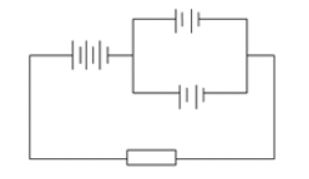
\includegraphics[scale=0.8]{../figs/VN12-Y21-PH-SYL-009-5.jpg}
		\end{center}
		\begin{mcq}(4)
			\item 0,5 A.
			\item 1 A.
			\item 2 A.
			\item 1,5 A.
		\end{mcq}
	}
	
	\loigiai{\textbf{Đáp án: B.}
		
		Xét đoạn mạch gồm 2 nhánh song song, mỗi nhánh gồm 2 nguồn nối tiếp ta có
		$$\calE_\text{ss} = 2\calE = 3\ \text{V}; r_\text{ss} = \dfrac{2r}{2} = 1\ \Omega.$$
		Đoạn mạch gồm 3 nguồn nối tiếp có 
		$$\calE_\text{nt} = 3\calE = \text{4,5}\ \text{V}; r_\text{nt} = 3r = 3\ \Omega.$$
		$$\Rightarrow \calE = \calE_\text{ss} + \calE_\text{nt} =\text{7,5}\ \text{V}; r_\text{b} =r_\text{ss} + r_\text{nt} =4\ \Omega.$$
		Cường độ dòng điện mạch ngoài là:
		$$I =\dfrac{\calE_\text{b}}{R+r_\text{b}} = 1\ \text{A}.$$
		
		
	}
	\item \mkstar{3}
	
	\cauhoi{Cần dùng bao nhiêu pin 4,5 V$-1\ \Omega$ mắc theo kiểu hỗn hợp để thắp cho bóng đèn 8 V - 8 W sáng bình thường?
		\begin{mcq}(4)
			\item 4.
			\item 5.
			\item 6.
			\item 7.
		\end{mcq}
	}
	
	\loigiai{\textbf{Đáp án: A.}
		
		Điện trở đèn:$$R =\dfrac{U^2}{\calP} =8\ \Omega.$$
		Giả sử pin mắc thành $n$ dãy song song mỗi dãy có $m$ nguồn ghép nối tiếp.
		
		Cường độ dòng điện đi qua mạch để đèn sáng bình thường là
		$$I=\dfrac{\calP}{U} = 1\ \text{A}.$$
		$$\Rightarrow I = \dfrac{\calE_\text{b}}{R+r_\text{b}} = \dfrac{m\calE}{8 + \dfrac{mr}{n}} = \dfrac{\text{4,5} mn}{m+8n} = \dfrac{\text{4,5}p}{m+8n} =1\ (1).$$
		Thay $n=\dfrac{p}{m}$ vào (1) ta có: 
		$$p = \dfrac{m^2}{\text{4,5}m -8}.$$
		Vì $p$ dương nên $m > \dfrac{16}{9}$ hay $m>1$.
		$$n = \dfrac{p}{m} \geq 1 \Leftrightarrow \dfrac{m^2}{\text{4,5}m-8}\geq 1.$$
		$$m \leq \text{2,3}.$$
		Suy ra $m=2, n=2$, có 4 pin. 
		
		
	}
	\item \mkstar{3}
	
	\cauhoi{Một bộ nguồn gồm 36 pin giống nhau ghép hỗn hợp thành $n$ hàng (dãy), mỗi hàng gồm $m$ pin ghép nối tiếp, suất điện động mỗi pin $\calE = 12\ \text{V}$, điện trở trong $r = 2\ \Omega$. Mạch ngoài có hiệu điện thế $U = 120\ \text{V}$ và công suất $P = 360\ \text{W}$. Khi đó $m, n$ bằng
		\begin{mcq}(2)
			\item $n = 12; m = 3$.
			\item $n = 3; m = 12$.
			\item $n = 4; m = 9$.
			\item $n = 9; m = 4$.
		\end{mcq}
	}
	
	\loigiai{\textbf{Đáp án: B.}
		
		Ta có: $$\calE_\text{b} = m\calE$$
		
		$$r_\text{b} =\dfrac{mr}{n}; R=\dfrac{U^2}{\calP} =40\ \Omega.$$
		Cường độ dòng điện trong mạch là
		$$I =\dfrac{\calE_\text{b}}{R+r_\text{b}} = \dfrac{\calP}{U} =3\ \text{A}$$
		Lại có: 
		$$mn=36 \Rightarrow n=3 \ \text{và}\ m =12$$
		
		
	}
	\item \mkstar{3}
	
	\cauhoi{Nguồn điện với suất điện động $\calE$, điện trở trong $r$, mắc với điện trở ngoài $R = r$, cường độ dòng điện trong mạch là $I$. Nếu thay nguồn điện đó bằng 3 nguồn điện giống hệt nó mắc nối tiếp thì cường độ dòng điện trong mạch là
		\begin{mcq}(4)
			\item $I'=3I$.
			\item $I'=2I$.
			\item $I'=\text{2,5}I$.
			\item $I'=\text{1,5}I$.
		\end{mcq}
	}
	
	\loigiai{\textbf{Đáp án: D.}
		
		Cường độ dòng điện trong mạch khi mắc một nguồn là
		$$I =\dfrac{\calE}{R+r} = \dfrac{\cal E}{2r}$$
		Khi thay bằng 3 nguồn giống nó mắc nối tiếp thì có $\calE' = 3\calE$; $r' = 3r$
		$$\Rightarrow I' = \dfrac{3\calE}{3+3r} = \dfrac{3\calE}{4r} \Rightarrow I'=\text{1,5}I.$$
		
		
	}
	\item \mkstar{3}
	
	\cauhoi{Một nguồn điện có suất điện động $\calE = \text{1,5}\ \text{V}$, điện trở trong $r= \text{0,1}\ \Omega$. Mắc giữa hai cực nguồn điện trở $R_1$ và $R_2$. Khi $R_1$ nối tiếp $R_2$ thì cường độ dòng điện qua mỗi điện qua mỗi điện trở là 1,5 A. Khi $R_1$ song song $R_2$ thì cường độ dòng điện tổng cộng qua 2 điện trở là 5 A. Giá trị của $R_1$ và $R_2$ bằng
		\begin{mcq}(2)
			\item $R_1= \text{0,2}\ \Omega; R_2= \text{0,9}\ \Omega$.
			\item $R_1= \text{0,4}\ \Omega; R_2= \text{0,5}\ \Omega$.
			\item $R_1= \text{0,6}\ \Omega; R_2= \text{0,3}\ \Omega$.
			\item $R_1= \text{0,2}\ \Omega; R_2= \text{0,7}\ \Omega$.
		\end{mcq}
	}
	
	\loigiai{\textbf{Đáp án: C.}	
		
		Khi $R_1$ nối tiếp $R_2$ thì cường độ dòng điện qua mỗi điện qua mỗi điện trở là
		$$I = \dfrac{\calE}{R_1+R_2+r} \Rightarrow R_1+R_2 = \text{0,9}.\ (*)$$
		Khi $R_1$ nối tiếp $R_2$ thì cường độ dòng điện tổng cộng qua 2 điện trở là
		$$I = \dfrac{\calE}{\dfrac{R_1R_2}{R_1+R_2}+r} \Rightarrow \dfrac{R_1R_2}{R_1+R_2} =\text{0,2}\  (**).$$
		Từ $(*)$ và $(**)$ ta tính được
		$$R_1= \text{0,6}\ \Omega; R_2= \text{0,3}\ \Omega.$$
		
		
		
	}
	\item \mkstar{3}
	
	\cauhoi{Nguồn điện có suất điện động $\calE$, điện trở trong $r$, mắc với điện trở ngoài $R=r$, cường độ dòng điện trong mạch là $I$. Nếu thay nguồn điện đó bằng 4 nguồn điện giống hệt nó mắc nối tiếp thì cường độ dòng điện trong mạch là
		\begin{mcq}(4)
			\item 1,5 $I$.
			\item 4$I$.
			\item 1,6$I$.
			\item 2$I$.
		\end{mcq}
	}
	
	\loigiai{\textbf{Đáp án: D.}
		
		Cường độ dòng điện trong mạch khi mạch chỉ có một nguồn
		$$I=\dfrac{\calE}{R+r} = \dfrac{\calE}{2R} .$$
		Thay nguồn điện trên bằng 3 nguồn điện giống nhau mắc nối tiếp thì suất điện động là $3\calE$, điện trở trong $3r$.
		
		Biểu thức cường độ dòng điện trong mạch là
		$$I'=\dfrac{4\calE}{R+3r} =\dfrac{4\calE}{4R}.$$
		Như vậy $$I'=2I.$$
		
		
	}
	\item \mkstar{4}
	
	\cauhoi{Cho mạch điện như hình vẽ. Hai pin có suất điện động bằng nhau và bằng $\calE_1=12\ \text{V}; \calE_2= 6\ \text{V}$, $r_1 = 3\ \Omega, r_2 = 5\ \Omega$. Hiệu điện thế giữa hai điểm A và B là
		\begin{center}
			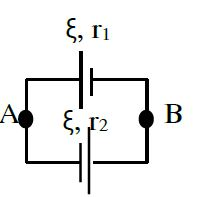
\includegraphics[scale=0.7]{../figs/VN12-Y21-PH-SYL-009-8.jpg}
		\end{center}
		\begin{mcq}(2)
			\item 1 A; 5 V.
			\item 0,75 A; 9,75 V.
			\item 3 A; 9 V.
			\item 2 A; 8 V.
		\end{mcq}
	}
	
	\loigiai{\textbf{Đáp án: B.}
		
		Cường độ dòng điện trong mạch:
		
		$$I = \dfrac{\calE_1 - \calE_2}{r_1 + r_2} = \text{0,75}\ \text{A}$$
		
		Suy ra hiệu điện thế giữa hai điểm A, B:
		$$U_\text{AB} = \calE_1 -Ir_1 =\text{9,75}\ \text{V}.$$
		
		
	}
	\item \mkstar{4}
	
	\cauhoi{Cho mạch điện như hình vẽ. Trong đó bộ nguồn gồm 8 Acquy, mỗi Acquy có suất điện động $\calE = 2\ \text{V}$, điện trở trong $r = \text{0,4}\ \Omega$ mắc thành hai nhánh, mỗi nhánh có 4 nguồn mắc nối tiếp; đèn loại 6 V - 6 W; $R_1 = \text{0,2}\ \Omega$; $R_2 =6\ \Omega$; $R_3 = 4\ \Omega$ và $R_4 =4\ \Omega$. Chọn phương án đúng.
		\begin{center}
			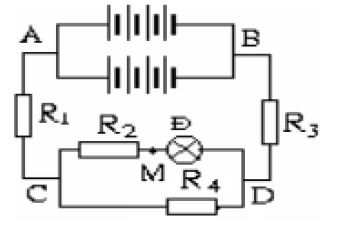
\includegraphics[scale=0.7]{../figs/VN12-Y21-PH-SYL-009-6.jpg}
		\end{center}
		\begin{mcq}(2)
			\item $U_\text{AM} = -\text{3,4}\ \text{V}$ và đèn sáng mạnh.
			\item $U_\text{AM} = \text{3,4}\ \text{V}$ và đèn sáng yếu.
			\item $U_\text{AM} = -\text{1,7}\ \text{V}$ và đèn sáng mạnh.
			\item $U_\text{AM} = \text{1,7}\ \text{V}$ và đèn sáng yếu.
			
		\end{mcq}
	}
	
	\loigiai{\textbf{Đáp án: D.}
		
		Ta có: $$P_\text{đ} = I^2_\text{đ}R_\text{đ} =\dfrac{U^2_\text{đ}}{R_\text{đ}} \Rightarrow R_\text{đ}= \dfrac{U^2_\text{đ}}{P_\text{đ}} = 6\ \Omega$$
		Phân tích: $R_1$ nt ($R_4\ //\ (R_2\text{ nt }R_\text{đ})\text{ nt } R_3$.
		$$R_\text{2đ} =R_2 +R_\text{đ} =12\ \Omega \Rightarrow R_\text{2đ4} = \dfrac{R_\text{2đ}R_4}{R_\text{2đ}+R_4} =3\ \Omega.$$
		$$\Rightarrow R = R_1 + R_\text{2đ4}+R_3 =\text{7,2}\ \Omega$$
		Mà $$\calE_\text{b} =4\calE =8\ \text{V}; r_\text{b}= \dfrac{4r}{2}=\text{0,8}\ \Omega.$$
		$$\Rightarrow I = \dfrac{\calE_\text{b}}{R+r_\text{b}} =1\ \text{A}$$
		Ta tính được:
		$$U_\text{AC} =IR_1 =\text{0,2}\ \text{V}.$$
		$$U_\text{CM} = I_\text{2đ}R_2 =\dfrac{U_\text{2đ}}{R_\text{2đ}}R_2 = \dfrac{U_\text{2đ4}}{R_\text{2đ}}R_2 =\dfrac{IR_\text{2đ4}}{R_\text{2đ}}R_2 =\text{1,5}\ \text{V}.$$
		Suy ra:
		$$U_\text{AM} = U_\text{AC} + U_\text{CM} = \text{1,7}\ \text{V}.$$ 
		
		
	}
	\item \mkstar{4}
	
	\cauhoi{Cho mạch điện như hình vẽ trong đó có 7 nguồn giống nhau, mỗi nguồn có suất điện động $\calE = 2\ \text{V}$, điện trở trong $r = \text{0,2}\ \Omega$ mắc như hình vẽ. Đèn có loại $\SI{6}{V} - \SI{12}{W}$; $R_1=\text{2,2}\ \Omega; R_2 = 4\ \Omega; R_3=2\ \Omega$. Hiệu điện thế $U_\text{MN}$ gần nhất với giá trị nào sau đây?
		\begin{center}
			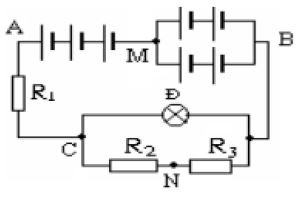
\includegraphics[scale=0.8]{../figs/VN12-Y21-PH-SYL-009-7.jpg}
		\end{center}
		\begin{mcq}(4)
			\item $-$ 4,2 V.
			\item 4,2 V.
			\item 2,3 V.
			\item $-$ 2,3 V.
		\end{mcq}
	}
	
	\loigiai{\textbf{Đáp án: C.}
		
		Ta có: $$\calE = 3\calE +2\calE =10\ \text{V}; r_\text{b} = 3r+ \dfrac{2r}{2} = \text{0,8}\ \Omega.$$
		$$R_\text{đ} = \dfrac{U^2_\text{đ}}{P_\text{đ}}=3\ \Omega.$$
		$$R_\text{23} = R_2+R_3 =6\ \Omega;$$
		$$R_\text{đ23} = \dfrac{R_\text{đ}R_{23}}{R_\text{đ}+R_{23}} =2\ \Omega.$$
		Điện trở toàn mạch:
		$$R=R_1+R_\text{đ23} =\text{4,2}\ \Omega.$$
		Cường độ dòng điện toàn mạch:
		$$I =\dfrac{\calE_\text{b}}{R+r_\text{b}} =2\ \text{A}$$
		Lại có:
		$$U_\text{đ23} = U_\text{đ} =U_{23} =IR_\text{Đ23} =4\ \text{V}.$$
		Suy ra:
		$$I_{23} = I_2=I_3 =\dfrac{U_{23}}{R_{23}} =\dfrac{2}{3}\ \text{A};$$
		Hiệu điện thế $U_\text{MN}$:
		$$U_\text{MN} =V_\text{M} - V_\text{N} = V_\text{M} - V_\text{C}+V_\text{C} - V_\text{N} = U_\text{MC} + U_\text{CN}.$$
		$$U_\text{MN} = I(3r+R_1)-3\calE + I_2R_2 =\text{2,3}\ \text{V}.$$
		
		
	}




	







\end{enumerate}

\whiteBGstarEnd

\loigiai{\begin{center}
		\textbf{BẢNG ĐÁP ÁN}
	\end{center}
	\begin{center}
		\begin{tabular}{|m{2.8em}|m{2.8em}|m{2.8em}|m{2.8em}|m{2.8em}|m{2.8em}|m{2.8em}|m{2.8em}|m{2.8em}|m{2.8em}|}
			\hline
			1.  C & 2.  B& 3.  A& 4.  B& 5.  B& 6.  A& 7.  B& 8.  C& 9.  A& 10.  C\\
			\hline
			11.  D& 12.  B& 13.  B& 14.  A& 15.  B& 16.  A& 17.  B& 18.  C& 19.  A& 20.  D\\
			\hline
			21. A & 22. D & 23. D & 24. C & 25. C & 26. B & 27. C & 28. A & 29. A & 30. B \\
			\hline
			31. D & 32. B & 33. A & 34. B & 35. D & 36. C & 37. D & 38. B & 39. D & 40. C \\
			\hline
		\end{tabular}
\end{center}}